% Clase del documento
\documentclass[12pt,twoside,titlepage]{report}


%%%%%%%%%%%%%%%%%%%%%%% Paquetes %%%%%%%%%%%%%%%%%%%%%%%

\usepackage[a4paper,bindingoffset=3mm,bottom=35mm]{geometry}


% Usad \usepackage[dvips]{graphicx} o \usepackage[pdftex]{graphicx} (no ambos)
%\usepackage[dvips]{graphicx} %%% para LaTeX. Las figuras deben estar en formato eps

\usepackage[colorlinks=true,pdftex]{hyperref}   %%% Opcional. Para incluir marcadores y enlaces en el pdf
\usepackage[pdftex]{graphicx}  %%% para pdflatex. Las figuras pueden estar en pdf, jpg, svg y otros formatos


\usepackage[spanish]{babel}

%\usepackage[latin1]{inputenc} % Usad en WinEdt/MikTex
\usepackage[utf8]{inputenc} % Usad en overleaf

%\usepackage[T1]{fontenc}


% Algunos paquetes útiles

\usepackage{amsmath,amssymb}
\usepackage{hyperref}
\usepackage{color}
\usepackage{afterpage}
\usepackage{paralist}
\usepackage{array}
\usepackage{enumerate}
\usepackage{paralist}
\usepackage{enumitem}
\usepackage{float}
\usepackage{setspace}
\usepackage{listings}
\usepackage{algorithm}
\usepackage{algorithmic}
\usepackage{fancyhdr}
\usepackage{rotating}
\usepackage{multirow}


% Otros paquetes

\usepackage{quotchap}
\usepackage{lipsum}

%%%%%%%%%%%%%%%%%%%%%%%%%%%%%%%%%%%%%%%%%%%%%%%%%%%%%%%%






%%%%%%%%%%%%%%%%%%%%%%% Definiciones básicas %%%%%%%%%%%%%%%%%%%%%%%

\newcommand{\nombreautor}{Sergio Simón Fernández}
\newcommand{\nombretutor}{Christian Alcaide Moreno}
\newcommand{\titulotrabajo}{Supercomparator}
\newcommand{\escuela}{IES Gabriel García Márquez}
\newcommand{\escuelalargo}{Escuela Técnica Superior de Ingeniería Informática}
\newcommand{\universidad}{XXX}
\newcommand{\fecha}{Fecha}
\newcommand{\grado}{Ciclo Formativo de Grado Superior en\\Desarrollo de Aplicaciones Multiplataforma}
\newcommand{\curso}{Curso 2022-2024}
\newcommand{\logoUniversidad}{logoURJC.pdf} % logoURJC.eps
\newcommand{\mercadonaPostman}{images/mercadona_postman.png} 
\newcommand{\mercadonaRequest}{images/mercadona_request.png} 
\newcommand{\superMasBarato}{images/super_mas_barato.png} 
\newcommand{\superMasBaratoBusqueda}{images/super_más_barato_result.png} 
\newcommand{\logIn}{images/login.png}
\newcommand{\soySuper}{images/soysuper.png} 
\newcommand{\register}{images/register.png}
\newcommand{\recoverAccount}{images/recover_account.png}
\newcommand{\recoverAccountCorreo}{images/correo_recuperacion.png}
\newcommand{\recoverAccountLink}{images/correo_recuperacion_2.png}
\newcommand{\kotlinMultiplataformSchema}{images/kotlin-multiplatform-structure.png}
\newcommand{\vico}{images/vico.png}
\newcommand{\spashScreen}{images/splash_screen.png}
\newcommand{\spalshScreenError}{images/spash_screen_error.png}
\newcommand{\spalshScreenSuccess}{images/splash_screen_success.png}
\newcommand{\annonSingin}{images/annon_login.png}
\newcommand{\correoSingin}{images/correo_singin.png}
\newcommand{\googleSingin}{images/gmail_singin.png}
\newcommand{\productScreen}{images/search_screen.png}
\newcommand{\productScreenResult}{images/search_result.png}
\newcommand{\favoriteScreen}{images/favorite_screen.png}
\newcommand{\cerrarSesion}{images/cerrar_sesion.png}
\newcommand{\productScreenSelected}{images/on_product_click.png}
\newcommand{\diagramaFlujo}{images/Supercomparator_diagrama.drawio.png}

%%%%%%%%%%%%%%%%%%%%%%%%%%%%%%%%%%%%%%%%%%%%%%%%%%%%%%%%%%%%%%%%%%%%






%%%%%%%%%%%%%%%%%%%%%%%%% Otras definiciones %%%%%%%%%%%%%%%%%%%%%%%%%%

% Definiciones de colores (para hidelinks)
%\definecolor{BlueLink}{rgb}{0.165,0.322,0.745}
% \definecolor{PinkLink}{rgb}{0.8,0.22,0.5}
% \definecolor{gray}{rgb}{0.6,0.6,0.6}


% Enlaces
\hypersetup{
    colorlinks=true,      % false: boxed links; true: colored links
    linkcolor=black,       % Color de los enlaces internos
    citecolor=cyan,      % Color de las citas
    filecolor=magenta,    % Color de los enlaces a archivos
    urlcolor=cyan         % Color de los enlaces externos
}

\newcommand\blankpage{%
    \newpage
    \null
    \thispagestyle{empty}%
    %\addtocounter{page}{-1}%
    \newpage}


% Texto referencias
\addto{\captionsspanish}{\renewcommand{\bibname}{Bibliografía}}

% Texto Índice de tablas
\addto\captionsspanish{
\def\tablename{Tabla}
\def\listtablename{\'{I}ndice de tablas}
}


\floatname{algorithm}{Algoritmo}

\newfloat{algorithm}{t}{lop}


%\newenvironment{pseudocodigo}[1][htb]
%  {\renewcommand{\algorithmcfname}{Pseudocódig}% Update algorithm name
%   \begin{algorithm}[#1]%
%  }{\end{algorithm}}
  
%%%%%%%%%%%%%%%%%%%%%%%%%%%%%%%%%%%%%%%%%%%%%%%%%%%%%%%%%%%%%%%%%%%%


%%%%%%%%%%%%%%%%%%%%%%% Estilo de código (en Koltin) %%%%%%%%%%%%%%%%%%%%%%%

\usepackage[dvipsnames]{xcolor}
\usepackage{listings}

\lstdefinelanguage{Kotlin}{
  comment=[l]{//},
  commentstyle={\color{gray}\ttfamily},
  emph={filter, first, firstOrNull, forEach, lazy, map, mapNotNull, println},
  emphstyle={\color{OrangeRed}},
  identifierstyle=\color{black},
  keywords={!in, !is, abstract, actual, annotation, as, as?, break, by, catch, class, companion, const, constructor, continue, crossinline, data, delegate, do, dynamic, else, enum, expect, external, false, field, file, final, finally, for, fun, get, if, import, in, infix, init, inline, inner, interface, internal, is, lateinit, noinline, null, object, open, operator, out, override, package, param, private, property, protected, public, receiveris, reified, return, return@, sealed, set, setparam, super, suspend, tailrec, this, throw, true, try, typealias, typeof, val, var, vararg, when, where, while},
  keywordstyle={\color{NavyBlue}\bfseries},
  morecomment=[s]{/*}{*/},
  morestring=[b]",
  morestring=[s]{"""*}{*"""},
  ndkeywords={@Deprecated, @JvmField, @JvmName, @JvmOverloads, @JvmStatic, @JvmSynthetic, Array, Byte, Double, Float, Int, Integer, Iterable, Long, Runnable, Short, String, Any, Unit, Nothing},
  ndkeywordstyle={\color{BurntOrange}\bfseries},
  sensitive=true,
  stringstyle={\color{ForestGreen}\ttfamily},
}

%%%%%%%%%%%%%%%%%%%%%%%%%%%%%%%%%%%%%%%%%%%%%%%%%%%%%%%%%%%%%%%%%%%%





%%%%%%%%%%%%%%%%%%%%%%% Estilo de código (en Python) %%%%%%%%%%%%%%%%%%%%%%%

\definecolor{bg}{rgb}{0.95,0.95,0.95}
\definecolor{mydeepteal}{rgb}{0.16,0.22,0.23}
\definecolor{myteal}{rgb}{0.31,0.44,0.46}
\definecolor{mymediumteal}{rgb}{0.41,0.58,0.60}

\DeclareFixedFont{\ttb}{T1}{txtt}{bx}{n}{12} % for bold
\DeclareFixedFont{\ttm}{T1}{txtt}{m}{n}{12}  % for normal


%\newcommand*{\FormatDigit}[1]{\textcolor{mydeepteal}{#1}}
\newcommand*{\FormatDigit}[1]{\textcolor{black}{#1}}

% Python style for highlighting
\newcommand\mypythonstyle{\lstset{
language=Python,
basicstyle=\ttfamily\small,
%basicstyle=\linespread{1.0}\footnotesize\ttm,
otherkeywords={self},             % Add keywords here
keywordstyle=\bfseries\ttfamily\color{myteal},
%keywordstyle=\ttb\color{myteal},
commentstyle=\itshape\color{myteal},
stringstyle=\color{mydeepteal},
emph={MyClass,__init__},          % Custom highlighting
emphstyle=\ttb\color{mydeepteal},    % Custom highlighting style
% Any extra options here
showstringspaces=false,            %
backgroundcolor=\color{bg},
rulecolor = \color{bg},
%identifierstyle=\color{deepgreen},
breaklines=true,
numbers=left,
numbersep=5pt,
numberstyle=\tiny,
tabsize=4,
xleftmargin=1em,
frame = single,
framesep = 3pt,
framextopmargin=0pt,
framexbottommargin=0pt,
framexleftmargin=0pt,
framexrightmargin=0pt,
fontadjust=true,
basewidth=0.55em, % compactness of code
upquote=true,
}}

% Python environment
\lstnewenvironment{mypython}[1][]
{
\mypythonstyle
\lstset{#1}
}
{}

\newcommand\mypythonstylenormalinline{\lstset{
language=Python,
basicstyle=\ttfamily\normalsize,
%basicstyle=\linespread{1.0}\footnotesize\ttm,
otherkeywords={self},            % Add keywords here
keywordstyle=\bfseries\ttfamily\color{myteal},
%keywordstyle=\ttb\color{myteal},
commentstyle=\itshape\color{mymediumteal},
stringstyle=\color{mydeepteal},
emph={MyClass,__init__},          % Custom highlighting
emphstyle=\ttb\color{mydeepteal},    % Custom highlighting style
% Any extra options here
showstringspaces=false,            %
backgroundcolor=\color{bg},
rulecolor = \color{bg},
%identifierstyle=\color{deepgreen},
breaklines=false,
numbers=left,
numbersep=5pt,
numberstyle=\tiny,
tabsize=4,
xleftmargin=0em,
frame = single,
framesep = 3pt,
framextopmargin=0pt,
framexbottommargin=0pt,
framexleftmargin=0pt,
framexrightmargin=0pt,
fontadjust=true,
%basewidth=0.55em, % compactness of code
upquote=true,
}}

\newcommand\mypythoninline[1]{{\mypythonstylenormalinline\lstinline!#1!}}

%%%%%%%%%%%%%%%%%%%%%%%%%%%%%%%%%%%%%%%%%%%%%%%%%%%%%%%%%%%%%%%%%%%%%%%%%%%%%%




%%%%%%%%%%%%%%%%%%%%%%%%%%%% Comandos definidos por el autor 

\newcommand{\transpuesta}{\mbox{\tiny $\mathsf{T}$}}








%%%%%%%%%%%%%%%%%%%%%%%%%%%%%%%%%%%%%%%%%%%%%%%%%%%%%%%%%%%%%%%%%%%%%%%
%                           Inicio del documento                       
%%%%%%%%%%%%%%%%%%%%%%%%%%%%%%%%%%%%%%%%%%%%%%%%%%%%%%%%%%%%%%%%%%%%%%%


\begin{document}

\pagestyle{plain}




%%%%%%%%%%%%%%%%%%%%%%%%%%%%%%%%%%%% Portada %%%%%%%%%%%%%%%%%%%%%%%%%%%%%%%%%%

%\pagenumbering{gobble}
%\pagenumbering{arabic}

% Universidad, Facultad
\begin{titlepage}
	\selectlanguage{spanish}


	% logo
	\begin{center}
		
\includegraphics[scale=1]{figuras/logo_ggm}
	\end{center}

	%\bigskip

	\begin{center}
		\begin{LARGE}
			\escuela \\
		\end{LARGE}
	\end{center}

	\bigskip
	\bigskip

	% Grado
	\begin{center}
		\begin{large}
			\textbf{\grado}\\
		\end{large}
	\end{center}

	% Curso
	\begin{center}
		\begin{large}
			\textbf{\curso}\\
		\end{large}
	\end{center}

	\bigskip

	\textbf{\begin{center}
			\begin{large}
				\textbf{Trabajo Fin de Ciclo}
			\end{large}
		\end{center}}

	\bigskip
	\bigskip
	\bigskip

	% Nombre del TFG
	\begin{center}
		\textbf{\begin{large}
				\MakeUppercase{\titulotrabajo}\\
			\end{large}}
	\end{center}

	% Nombre del autor
	\vspace{\fill}
	\begin{center}
		\textbf{Autor: \nombreautor}\\ \smallskip
		% Tutor
		\textbf{Tutor: \nombretutor}\\
		% Añadir segundo tutor si hubiera


		\bigskip

		% Fecha
		%\textbf{\fecha}\\
	\end{center}
\end{titlepage}


%%%%%%%%%%%%%%%%%%%%%%%% Opcional %%%%%%%%%%%%%%%%%%%%%%
%\blankpage

%\thispagestyle{empty}
%\begin{center}

% Nombre del trabajo
%\textbf{\begin{large}
%\MakeUppercase{\titulotrabajo}\\*
%\end{large}}
%\vspace*{0.2cm}
%\vspace{5cm}

% Nombre del autor y del tutor
%\large Autor: \nombreautor \\* \medskip
%\large Tutor: \nombretutor \\*

%\vfill

% Escuela, universidad y fecha
%\escuelalargo \\ \smallskip
%\universidad \\
%\vspace{1cm}
%\fecha \\

%\clearpage

%\end{center}
%%%%%%%%%%%%%%%%%%%%%%%%%%%%%%%%%%%%%%%%%%%%%%%%%%%%%%%%

\hypersetup{pageanchor=true}

\normalsize
\afterpage{\blankpage} % Se deben añadir página en blanco para que lo capítulos de la memoria o estas secciones introductorias empiecen en páginas impares

%%%%%%%%%%%%%%%%%%%%%%%%%%%%%%%%%%%%%%%%%%%%%%%%%%%%%%%%%%%%%%%%%%%%%%%%%%%%%%%





% Estilo de párrafo de los capítulos
\setlength{\parskip}{0.75em}
\renewcommand{\baselinestretch}{1.25}
% Interlineado simple
\spacing{1}

\pagenumbering{Roman}
\setcounter{page}{2}


%%%%%%%%%%%%%%%%%%%%%%%%% Agradecimientos o dedicatoria %%%%%%%%%%%%%%%%%%%%%%%%%%%

\chapter*{Agradecimientos}

Quisiera agradecer a todo el equipo docente, del \escuela por la gran labor que han realizado durante este curso, en especial a mi tutor de proyecto Christian, por la ayuda y los consejos que me ha ofrecido durante todo el proceso.

\afterpage{\blankpage}

%%%%%%%%%%%%%%%%%%%%%%%%%%%%%%%%%%%%%%%%%%%%%%%%%%%%%%%%%%%%%%%%%%%%%%%%%%%%%%%%%%%






%%%%%%%%%%%%%%%%%%%%%%%%%%%%%%%%%%%% Resumen %%%%%%%%%%%%%%%%%%%%%%%%%%%%%%%%%%%%%%

\chapter*{Resumen}

Se propuso desarrollar una aplicación multiplataforma para obtener información de productos en distintos supermercados y comparar sus precios. La aplicación permitiría la búsqueda simultánea de varios productos, con funciones adicionales como iniciar sesión y guardar productos.

El objetivo era crear una herramienta útil para los consumidores, ayudándoles a tomar decisiones informadas y económicas. Los usuarios podrían ingresar a la aplicación, buscar productos en diferentes supermercados y comparar precios detalladamente. También se incluiría el historial de precios y la opción de añadir productos a una lista de favoritos.

Durante el desarrollo, se identificaron desafíos significativos. Se concluyó que el desarrollo multiplataforma no era viable debido a limitaciones técnicas y de recursos, lo que llevó a enfocar el proyecto en una sola plataforma para asegurar una implementación sólida. Además, se experimentaron retrasos que impidieron la implementación de consultas múltiples.

A pesar de estos contratiempos, se lograron alcanzar otros objetivos clave. La aplicación permite a los usuarios iniciar sesión, guardar productos de interés y acceder a información detallada de precios en diferentes supermercados.

En resumen, aunque no se pudo desarrollar la funcionalidad multiplataforma ni las consultas múltiples, el proyecto avanzó significativamente en otras áreas importantes, proporcionando una herramienta eficaz para la comparación de precios y ayudando a los usuarios a ahorrar tiempo y dinero en sus compras diarias.

\mbox{} \smallskip

\noindent \textbf{Palabras clave}:
\begin{compactitem}
	\item Web scraping
	\item Multiplataforma
	\item API REST
    \item Asincronía
    \item Clean code
    \item Clean arquitecture
    \item Kotlin
    \item Java
    \item JavaScript
    \item MVVM (Model View, View, Model)
\end{compactitem}

\afterpage{\blankpage}

%%%%%%%%%%%%%%%%%%%%%%%%%%%%%%%%%%%%%%%%%%%%%%%%%%%%%%%%%%%%%%%%%%%%%%%%%%%%%%%%%%%





%%%%%%%%%%%%%%%%%%%%%%%%%%%%%%%%%%%% Índices %%%%%%%%%%%%%%%%%%%%%%%%%%%%%%%%%%%%

% Estilo de párrafo de los Índices
\setlength{\parskip}{1pt}
\renewcommand{\baselinestretch}{1}
\renewcommand{\contentsname}{Índice de contenidos}


% Índice de contenidos
\tableofcontents
\afterpage{\blankpage}

% Índice de figuras (OPCIONAL)
\listoffigures
\afterpage{\blankpage}
\addcontentsline{toc}{chapter}{\listfigurename}

% Índice de códigos/algoritmos (OPCIONAL).   El término "Códigos" se puede cambiar por "Métodos", "Funciones", "Algoritmos", etc.
\renewcommand\lstlistlistingname{Códigos}
\renewcommand\lstlistingname{Código}
\renewcommand\lstlistlistingname{Índice de códigos}

\lstlistoflistings
\afterpage{\blankpage}
\addcontentsline{toc}{chapter}{\lstlistlistingname}


% En este documento (de momento) no se ha considerado incluir un índice de algoritmos/pseudocódigos, como el que aparece en \ref{AdditionalLouvain}

%%%%%%%%%%%%%%%%%%%%%%%%%%%%%%%%%%%%%%%%%%%%%%%%%%%%%%%%%%%%%%%%%%%%%%%%%%%%%%%%%%%





%%%%%%%%%%%%%%%%%%%%%%% Cabeceras y pies de página (Opcional) %%%%%%%%%%%%%%%%%%%%%%%

%\setlength{\headheight}{15.2pt}
\pagestyle{fancy}


\renewcommand{\chaptermark}[1]{\markboth{Capítulo \thechapter.\ #1}{}}

\pagestyle{fancy}
\fancyhf{}
\fancyhead[LO]{\leftmark}
\fancyhead[RO]{}
\fancyhead[RE]{\nouppercase\rightmark}
\fancyhead[LE]{}
\fancyfoot[C]{\thepage}

%%%%%%%%%%%%%%%%%%%%%%%%%%%%%%%%%%%%%%%%%%%%%%%%%%%%%%%%%%%%%%%%%%%%%%%%%%%%%%%%%%%%






%%%%%%%%%%%%%%%%%%%%%%%%%%%%%% Capítulos de la memoria %%%%%%%%%%%%%%%%%%%%%%%%%%%%%



% Capítulo 1
\chapter{Introducción}


%%%%%%%%%%%%%%%%%%%%%%%%%%%%%%%%%%%%%%%%%%%%%%%%%%%%%%%%%%%%%%%%%%%%%%%%%%

% Estilo resto de páginas
\pagestyle{fancy}


% Estilo de párrafo de los capítulos
\setlength{\parskip}{0.75em}
\renewcommand{\baselinestretch}{1.25}
% Interlineado simple
\spacing{1}
% Numeración contenido
\pagenumbering{arabic}
\setcounter{page}{1}

%%%%%%%%%%%%%%%%%%%%%%%%%%%%%%%%%%%%%%%%%%%%%%%%%%%%%%%%%%%%%%%%%%%%%%%%%%

En este capítulo se desarrolla una pequeña introducción a la estructura de la memoria, se contará de que va a ir cada capítulo, brevemente situando al lector de que trata cada punto y se pondrá en contexto de que trata el proyecto 

\section{Estructura del documento}

La memoria del proyecto posee seis apartados diferenciados:

\begin{itemize}
\item[1] \textbf{Introducción}: \\ Se sitúa al lector proporcionando el contexto necesario para comprender el propósito y la idea central del proyecto. En esta sección se describen los puntos que se van a tratar y se explica el alcance del proyecto.

\item[2] \textbf{Objetivos}: \\ Se redactan los hitos que se proponen alcanzar durante el desarrollo del proyecto. Se establece un objetivo general que resume la funcionalidad global del proyecto, desarrollando más a fondo las funcionalidades específicas en los objetivos específicos.

\item[3] \textbf{Estado del arte}: \\ Se realiza una comparación de proyectos similares, analizando sus características y los criterios tomados en cuenta para el desarrollo del proyecto.

\item[4] \textbf{Metodología}: \\ Se narra cómo se ha desarrollado el proyecto, incluyendo los conocimientos relacionados con los módulos que han servido para su desarrollo. Se define las tecnologías usadas y se detalla el proceso de desarrollo del proyecto.

\item[5] \textbf{Resultados y discusión}: \\ Se reflexiona sobre lo que ha supuesto el desarrollo del proyecto y se discuten las posibles mejoras.

\item[6] \textbf{Conclusiones}: \\ Se repasan los aspectos que han funcionado en el proyecto y los que no. Se analizan los errores y aciertos durante el desarrollo del proyecto.
\end{itemize}

\section{Contexto y alcance}

En los últimos años, hemos notado un aumento considerable en el costo de vida, en especial cuando hacemos nuestras compras diarias. Al ir de compras, siempre buscamos los lugares más económicos para ahorrar dinero. Sin embargo, debido a la gran cantidad de supermercados y la diversidad de productos disponibles en la actualidad, esta tarea puede resultar tediosa y consumir mucho tiempo.

Para abordar esta problemática, se decidió desarrollar la aplicación SuperComparator. Esta herramienta permite comparar precios de manera sencilla e intuitiva, facilitando así el ahorro de tiempo, esfuerzo y dinero. Con SuperComparator, los usuarios podrán encontrar rápidamente las mejores ofertas y tomar decisiones informadas sobre dónde realizar sus compras, optimizando sus decisiones y mejorando su experiencia de compra.

% Capítulo 2
\chapter{Objetivos}

En este capítulo se desarrollan los principales objetivos del proyecto indicando cuál es la principal funcionalidad que debe realizar la aplicación y posteriormente detallando con más detenimiento los detalles más específicos que se deben realizar


% Objetivos generales y específicos del trabajo.


\section{Objetivo general}

Desarrollar una aplicación en Android capaz de comparar precios de distintos supermercados y recopilar un historial de precios.

\section{Objetivos específicos}

\begin{itemize}

	\item[1] Obtener productos de distintos supermercados.
 
	\item[2] Permitir registro e inicio de sesión online.
 
    \item[3] Permitir la realización de búsqueda de productos de manera individual.
	
    \item[4] Permitir de manera automatizada varias consultas de distintos productos.
	
    \item[5] Agregar productos a una lista de favoritos.
	
    \item[6] Permitir a los usuarios ver información detallada de los productos como su precio histórico o el precio por unidad.

    \item[7] Diseñar una interfaz atractiva.

    \item[8] Emplear un diseño minimalista 

    \item[9] Diseñar una interfaz intuitiva y reconocible
    
\end{itemize}

\blankpage


% Capítulo 3
\chapter{Estado del arte}

En este capítulo, exploraremos diversas herramientas disponibles en el mercado, detallando sus funcionalidades y características. Evaluaremos cuáles de estas características son comunes con nuestro proyecto y cuáles no. Este análisis permitirá comparar otras alternativas e identificar innovaciones en nuestro proyecto en relación con desarrollos previos. Además, nos servirá de inspiración para futuras versiones del proyecto, tomando lo mejor de cada herramienta.

\section{Súper más barato}

Súper más barato \cite{Super más barato} permite elegir los supermercados en los que se desea comparar los precios de los productos. Al realizar una búsqueda, se mostrará el nombre del producto, una imagen del mismo, su precio y el precio por unidad.

Súper Más Barato es una página web, a diferencia del proyecto que está desarrollado en Android. \titulotrabajo ofrece una búsqueda de productos por tienda, muy similar a Súper Más Barato. Sin embargo, en Súper Más Barato no es posible elegir el filtro de precio, añadir productos a una lista de favoritos o ver su historial de precios.

\begin{figure}[H]
    \centering
	\includegraphics[width=0.80\textwidth,clip=true]{\superMasBarato}
    \caption{Web Super Más Barato}
    \label{fig:superMasBarato}
\end{figure}

\begin{figure}[H]
    \centering
	\includegraphics[width=0.80\textwidth,clip=true]{\superMasBaratoBusqueda}
    \caption{Web Super Más Barato Búsqueda}
    \label{fig:superMasBarato}
\end{figure}

\section{Soysuper}

Soysuper \cite{Soysuper} es una web que cuenta con aplicaciones disponibles tanto para Android como iOS. Aunque ofrece las funciones básicas de búsqueda y comparación entre supermercados, destaca por una característica innovadora: la posibilidad de agregar productos a la cesta del supermercado directamente desde su página web. Actualmente, esta función solo está disponible para productos de la misma cadena de supermercados. Otra característica notable es la presencia de una variedad de productos recomendados, sin necesidad de realizar búsquedas previas, lo que sugiere la existencia de una base de datos propia que abarca todos los productos de los supermercados, o al menos, de búsquedas anteriores.

Soysuper posee la característica única de añadir productos a la cesta de supermercados, funcionalidad que no está presente en el proyecto. Sin embargo, a diferencia de Soysuper, el proyecto tiene la capacidad de almacenar un historial de precios y añadir productos a una lista de favoritos.

\begin{figure}[H] % Usar [H] para forzar la posición exacta
    \centering
    \includegraphics[width=1.00\textwidth]{images/soySuper.png}
    \caption{Web SoySuper}
    \label{fig:soySuper}
\end{figure}


% Capítulo 4
\chapter{Metodología}
\label{chap:contenidos}

En este capítulo, se detallan las metodologías utilizadas en el proyecto, su relación con los ciclos impartidos durante el curso, sus puntos en común y cómo han contribuido al desarrollo del proyecto. Se describirán las tecnologías empleadas, su papel en el proyecto y se proporcionará una definición de cada una. Además, se narrará el proceso de desarrollo del proyecto, incluyendo las complicaciones encontradas y los detalles del desarrollo, justificando las decisiones tomadas.

\section{Relación con el Ciclo}

El proyecto está estrechamente vinculado con las materias de aplicaciones móviles, programación de procesos y acceso a datos.

La aplicación, desarrollada para Android, se fundamenta en los conocimientos adquiridos en clase. Sin embargo, se decidió utilizar Compose como alternativa a la construcción de vistas mediante XML. Además, se adoptó un enfoque orientado a la arquitectura de código, implementando el patrón MVVM (Model-View-ViewModel). Se exploraron librerías como Firebase para la autenticación, Retrofit para las solicitudes de red y Coil como evolución de Picasso para proporcionar imágenes de manera offline.

En la asignatura de programación de procesos, se aplicaron los conocimientos sobre hilos para realizar consultas asíncronas entre diferentes tiendas, reduciendo así el tiempo de espera entre las solicitudes. También se desarrolló una API Rest con Spring Boot, investigando su funcionamiento y buscando formas más eficientes y legibles de desarrollar código, utilizando principios de Clean Code y una arquitectura hexagonal.

En la materia de acceso a datos, se emplearon los conocimientos sobre filtrado y obtención de datos de archivos JSON y XML. Además, se ampliaron estos conocimientos con el uso de bases de datos no relacionales, específicamente MongoDB.

\section{Introducción a la Tecnología/Aplicación utilizada}

A continuación se describirán las tecnologías más destacables usadas en el proyecto y que parte han desempeñado para su realización 

\subsection{Kotlin Multiplataform}
\label{sec:Kotlin-Multiplataform}

En la página oficial de Kotlin \cite{kotlin-multiplataform}, se define a Kotlin Multiplatform como una tecnología diseñada para reducir el tiempo en proyectos multiplataforma. Esto se logra disminuyendo el tiempo dedicado a escribir y mantener el mismo código para diferentes plataformas, al tiempo que se conserva la flexibilidad y los beneficios de la programación nativa.

Kotlin Multiplatform permite mantener una única base de código para la lógica de la aplicación en diversas plataformas. Además, ofrece las ventajas de la programación nativa, incluido un excelente rendimiento y acceso completo a los SDK de cada plataforma.

\begin{figure}[H]
    \centering
    \includegraphics[width=0.85\textwidth,clip=true]{\kotlinMultiplataformSchema}
    \caption{Kotlin Multiplataform Schema}
    \label{fig:kotlinMultiplataformSchema}
\end{figure}

\subsection{Retrofit}
\label{sec:Retrofit}

Retrofit \cite{retrofit} es una biblioteca para Android y Java desarrollada por Square que facilita la creación de clientes HTTP para consumir APIs RESTful. Simplifica las tareas de realizar solicitudes HTTP, como GET, POST, PUT y DELETE, al convertir automáticamente las respuestas JSON o XML en objetos Java o Kotlin, utilizando convertidores específicos. 

\subsection{MongoDB}
\label{sec:MongoDB}

MongoDB \cite{mongodb} es una base de datos NoSQL orientada a documentos, desarrollada por MongoDB Inc., que se utiliza para almacenar y gestionar grandes volúmenes de datos de manera flexible y escalable. A diferencia de las bases de datos relacionales tradicionales que almacenan datos en tablas con filas y columnas, MongoDB almacena datos en documentos BSON (una extensión binaria de JSON), permitiendo una estructura de datos más dinámica y ágil.

\subsection{Web scraping}
\label{sec:WebScraping}

Para el proyecto \titulotrabajo \space se ha sido necesario el uso \textbf{web scraping}, según la página web Geeksforgeeks define WebScraping \cite{WebScraping} de la siguiente manera:

\begin{itemize}
	\item Imaginemos que necesitas obtener información de un sitio web. Copiar y pegar puede servir para pequeñas cantidades, pero ¿qué hacer si requieres grandes cantidades de datos de manera rápida? En ese caso, copiar y pegar simplemente no es una opción viable. Ahí es donde entra en juego el Web Scraping. A diferencia del tedioso proceso manual de recopilación de datos, el Web Scraping emplea técnicas automatizadas para extraer miles o incluso millones de conjuntos de datos en un lapso de tiempo mucho más corto.
\end{itemize}

En el proyecto se han utilizado dos métodologias de web scraping:

\begin{itemize}
	\item Llamado de una api del comercio

    Cuando se solicitan datos al api del comercio, estos llegan en formato json, describiendo los productos consultados. A partir de esta información, se realiza una conversión a un objeto Kotlin. Este objeto almacena la información completa o parcial del producto, dependiendo del alcance de la consulta y la relevancia de los datos obtenidos.
 
	\item Filtrado del html del comercio

    El proceso de filtrado mediante html es bastante similar. Se realiza una consulta que devuelve todo el contenido de la página web del comercio. A continuación, se trabaja con este html para extraer los datos relevantes y almacenarlos en un objeto Kotlin. Este filtrado se lleva a cabo utilizando las etiquetas html, asociadas a clases css, que permiten   distinguir los distintos campos de la página y extraer los datos necesarios.
\end{itemize}

\subsection{Selenium WebDriver}

\label{sec:Selenium}

Selenium WebDriver, según la página web \textit{El blog de python} \cite{Selenium WebDriver} es una herramienta de automatización de pruebas que permite interactuar con aplicaciones web de forma automatizada.

La elección de Selenium WebDriver se fundamenta en su funcionamiento interno. Esta herramienta opera mediante un controlador de navegador, como Firefox, para ejecutar las pruebas de forma automática. Crea un navegador virtual que permite ejecutar el JavaScript necesario en aquellas páginas que requieren este tipo de interacción.

Este enfoque ha permitido realizar consultas a las páginas web de Hipercor y Mercadona. En el caso de Hipercor, su API siempre devolvía un error 404 al utilizar Retrofit (véase \ref{sec:Retrofit}). Con Mercadona, el problema surgía porque, al hacer una llamada HTTP simple para obtener su HTML, la respuesta incluía un error indicando que no se pudo ejecutar el código JavaScript. Para solucionar esto, se ha utilizado Selenium para emular un navegador y hacer scraping de su contenido en HTML (véase la sección \ref{sec:WebScraping}).

\subsection{Firebase}
\label{sec:Firebase}

\textbf{Firebase} \cite{Firebase} es una plataforma para el desarrollo de aplicaciones web y móviles que permite a los desarrolladores ahorrar tiempo en la programación. Ofrece soluciones multiplataforma (iOS, Android, Unity, etc.) y cuenta con la infraestructura de Google, lo que permite escalar automáticamente a medida que la aplicación crece. Además, Firebase permite medir el rendimiento del proyecto mediante Firebase Analytics.

Ente sus herramientas se encuentra: 

\begin{itemize}

\item \textbf{Firebase Cloud Messaging} \\
Firebase Cloud Messaging (FCM) es un servicio que permite enviar notificaciones y mensajes a aplicaciones móviles y web sin costo alguno. FCM soporta distintos tipos de mensajes, incluyendo notificaciones que pueden mostrarse al usuario y datos que la aplicación puede manejar de forma silenciosa en el fondo. Es ideal para alertar a los usuarios sobre nuevos eventos, actualizaciones de contenido, mensajes personales, y más, con opciones de envío segmentado basadas en temas, grupos de dispositivos o usuarios individuales.

\item \textbf{Firebase Auth} \\
Firebase Authentication proporciona una forma rápida y segura de manejar la autenticación de usuarios en aplicaciones. Admite varios métodos de autenticación, incluyendo correo electrónico y contraseña, proveedores de identidad federada como Google, Facebook y Twitter, así como métodos anónimos. Firebase Auth facilita la implementación de flujos de inicio de sesión y registro, y se integra con otros servicios de Firebase para brindar una experiencia de usuario unificada y segura.

\item \textbf{Firebase Database} \\
Firebase Realtime Database es una base de datos NoSQL alojada en la nube que permite almacenar y sincronizar datos entre usuarios en tiempo real. Todos los datos se almacenan en formato JSON y se sincronizan en tiempo real a cada cliente conectado. Es ideal para aplicaciones colaborativas como chats, juegos en línea y aplicaciones que requieren datos en tiempo real. Ofrece funcionalidades como el almacenamiento sin conexión, lo que permite que las aplicaciones sigan funcionando y se sincronicen cuando la conexión se restablezca.

\item \textbf{Firebase Storage} \\
Firebase Storage ofrece una solución robusta y escalable para almacenar y servir archivos generados por usuarios, como fotos, videos y otros contenidos multimedia. Está construido sobre Google Cloud Storage, garantizando una alta disponibilidad y escalabilidad. Firebase Storage maneja de forma segura las subidas y descargas de archivos, y se integra fácilmente con Firebase Authentication para permitir el control de acceso basado en los usuarios. Proporciona capacidades de reanudación de cargas y descargas, lo que mejora la experiencia del usuario en redes inestables.

\item \textbf{Firebase Cloud Firestore} \\
Firebase Cloud Firestore es una base de datos flexible y escalable para desarrollo móvil, web y servidor. Es una base de datos NoSQL que permite el almacenamiento, la sincronización y la consulta de datos de aplicaciones a una escala global. Firestore ofrece consultas sofisticadas, estructura de datos en tiempo real y soporte para transacciones. A diferencia de Realtime Database, Firestore tiene una estructura jerárquica y soporta colecciones y documentos anidados, lo que facilita la organización y consulta de datos complejos. También se sincroniza en tiempo real y ofrece capacidades sin conexión, asegurando que las aplicaciones funcionen de manera eficiente en cualquier circunstancia de conectividad. \\

Cada uno de estos módulos proporciona herramientas esenciales para desarrollar aplicaciones robustas y eficientes, permitiendo a los desarrolladores centrarse en la lógica de negocio sin preocuparse por la infraestructura subyacente.

Se han utilizado principalmente las funcionalidades de autenticación que proporciona Firebase, incluyendo correo/contraseña, usuario anónimo y cuenta de Google. Además, se han implementado las analíticas de Firebase para recopilar información sobre el uso de la aplicación por parte de los usuarios.

\end{itemize}

\subsection{Spring Boot}
\label{sec:Springboot}

Spring Boot \cite{springboot-ibm} \cite{springboot-baeldung} es una extensión del popular marco de trabajo empresarial Java Spring Framework. Se destaca por su capacidad para simplificar y acelerar el desarrollo de microservicios y aplicaciones web. Spring Boot se distingue por tres características principales:

\textbf{1. Configuración automática}: Spring Boot ofrece una configuración automática inteligente que detecta las dependencias en el proyecto y configura automáticamente la aplicación en consecuencia. Esto reduce significativamente la cantidad de configuración manual necesaria para poner en marcha una aplicación.

\textbf{2. Enfoque de configuración obstinado}: Spring Boot promueve un enfoque de configuración obstinado, lo que significa que proporciona valores predeterminados sensatos para la configuración, pero permite a los desarrolladores anular estos valores fácilmente cuando sea necesario. Esto proporciona flexibilidad para adaptar la configuración según los requisitos específicos del proyecto.

\textbf{3. Capacidad de crear aplicaciones autónomas}: Una de las características más destacadas de Spring Boot es su capacidad para generar aplicaciones autónomas. Esto significa que una aplicación Spring Boot puede empaquetar todo lo que necesita para ejecutarse, incluida la máquina virtual Java (JVM), lo que la hace independiente de la instalación de software adicional en el entorno de ejecución. Esta característica simplifica enormemente la implementación y el despliegue de aplicaciones.

En conjunto, estas características hacen de Spring Boot una herramienta poderosa para el desarrollo rápido y eficiente de aplicaciones Java, permitiendo a los desarrolladores enfocarse en la lógica de la aplicación en lugar de preocuparse por la configuración y el entorno de ejecución.


\subsection{Jetpack Compose}
\label{sec:Jetpack Compose}

Jetpack Compose es un moderno kit de herramientas de UI (Interfaz de Usuario) para la construcción de interfaces de aplicaciones de Android de manera declarativa y con un enfoque basado en componentes. Desarrollado por Google, se integra con el ecosistema de Jetpack de Android y está diseñado para simplificar y acelerar el desarrollo de aplicaciones Android mediante la adopción de patrones de diseño más intuitivos y eficientes.

En lugar de utilizar XML para definir la interfaz de usuario, Jetpack Compose utiliza Kotlin, lo que permite a los desarrolladores describir la interfaz de usuario de manera más concisa y dinámica mediante funciones y composiciones de componentes. Esto facilita la creación de interfaces de usuario altamente personalizadas y adaptables, además de simplificar tareas como la gestión del estado de la interfaz de usuario y la interacción con los datos.

Jetpack Compose ofrece una experiencia de desarrollo más fluida al proporcionar herramientas de previsualización en tiempo real, lo que permite a los desarrolladores ver instantáneamente cómo se verán y se comportarán los cambios en la interfaz de usuario mientras escriben código. Además, está diseñado para ser compatible con las herramientas y bibliotecas existentes de Android, lo que facilita la integración en proyectos de Android existentes y la adopción gradual en nuevas aplicaciones.

La interfaz de la aplicación está realizada enteramente con Jetpack Compose, utilizando los componentes de Material 3 para darle un aspecto moderno y actual. La interfaz ha sido diseñada teniendo en cuenta el modo oscuro de los teléfonos, adaptándose automáticamente al tema del sistema. Además, en dispositivos con Android 13, la aplicación soporta los temas dinámicos del sistema.

\subsection{Coil}
\label{sec:Coil}

Coil es una librería para la carga y manipulación de imágenes en aplicaciones Android. Permite almacenar en la caché del sistema las imágenes consultadas en internet, facilitando así su carga de manera offline.

\subsection{Arquitectura Hexagonal}
\label{sec:Arquitectura Hexagonal}

La arquitectura hexagonal\cite{arquitectura-hexagonal} es un modelo de diseño de aplicaciones de software en torno a la lógica de dominio para aislarla de factores externos.

La lógica del dominio se especifica en un núcleo de negocio, al que llamaremos la parte interna, mientras que el resto son partes externas. El acceso a la lógica del dominio desde el exterior está disponible a través de puertos y adaptadores.

La arquitectura hexagonal define la interna y exterior. Se dividen en tres capas:

\begin{itemize}
    \item Aplicación (Exterior)
    \item Dominio (Interior)
    \item Infraestructura (Exterior)
\end{itemize}

A través de la capa de aplicación, el usuario u otros programas interactúan con la aplicación. Esta capa debe contener elementos como interfaces de usuario, controladores RESTful y bibliotecas de serialización JSON. Incluye todo lo necesario para exponer el acceso a la aplicación y organizar la ejecución de la lógica del dominio.

En la capa de dominio, se mantiene el código que implementa la lógica empresarial. Esta es el núcleo de la aplicación. Esta capa debe estar aislada tanto de la capa de aplicación como de la capa de infraestructura. Además, debe contener interfaces que definan la API para comunicarse con partes externas, como la base de datos, con la que interactúa el dominio.

Finalmente, la capa de infraestructura contiene todo lo que la aplicación necesita para funcionar, como la configuración de la base de datos o la configuración de Spring. También implementa las interfaces dependientes de la infraestructura definidas en la capa de dominio.

Este enfoque permite separar el trabajo en cada capa. Podemos enfocarnos en una capa sin afectar a las demás.

Además, estas capas son naturalmente más fáciles de entender por qué cada una se centra en su propia lógica.

Otra gran ventaja es que la lógica del dominio está aislada de todo lo demás. La parte del dominio solo contiene la lógica empresarial y se puede mover fácilmente a un entorno diferente.

\subsection{Vico}
\label{sec:vico}

La librería Vico para Android es una biblioteca gráfica de código abierto diseñada para facilitar la creación de gráficos y visualizaciones de datos en aplicaciones Android. Desarrollada por Javiersc, Vico proporciona una API intuitiva y flexible que permite a los desarrolladores integrar diversos tipos de gráficos, como gráficos de líneas, gráficos de barras, y otros tipos de visualizaciones, de manera rápida y eficiente.

\begin{figure}[H]
    \centering
	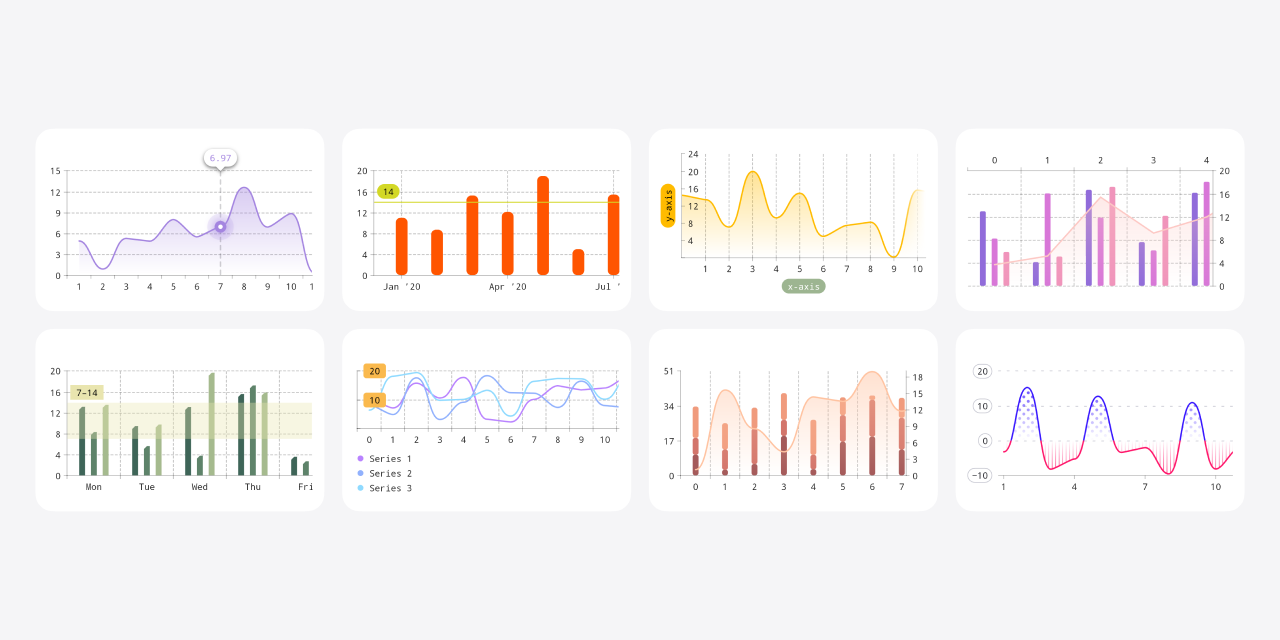
\includegraphics[width=1.00\textwidth,clip=false]{\vico}
    \caption{Vico Gráficos}
    \label{fig:Log-In}
\end{figure}


\section{Desarrollo del proyecto}

Para el desarrollo del proyecto, inicialmente se consideró utilizar Kotlin Multiplatform (véase \ref{sec:Kotlin-Multiplataform}). Sin embargo, como se detalla en \ref{sec:Mal-Kotlin-Multiplataforma}, esto resultó ser un gran desafío. La dificultad de encontrar bibliotecas compatibles, configurarlas y buscar equivalentes multiplataforma para muchos elementos de Compose retrasó significativamente el desarrollo. Debido a estos problemas, se decidió migrar el proyecto a Android usando Compose, ya que en Android sí existe una documentación detallada.

Una vez migrado el código a Android, que inicialmente solo incluía las vistas de inicio de sesión y registro, el desarrollo del proyecto avanzó más rápidamente. Durante esta fase, se investigó y ajustó la interfaz para desarrollar un estilo propio en la app y se exploraron métodos para implementar nuevos elementos. Además, se investigaron diversas formas de hacer scraping para extraer la información de las tiendas (véase \ref{sec:WebScraping}).

No había una manera estándar para acceder a la información, como se detalla en \ref{sec:Mal-Consultas}, lo que resultó en que cada comercio tuviera sus propias particularidades e inconvenientes. Por ejemplo, Mercadona no tenía una API pública y no se podía acceder de manera estándar con simples peticiones HTTP utilizando alguna librería como Retrofit (véase \ref{sec:Retrofit}). Para solucionar esto, se usó la librería Selenium (véase \ref{sec:Selenium}), que emula un navegador para automatizar tareas y puede ejecutar JavaScript, lo cual es necesario para poder hacer peticiones a la tienda de Mercadona.

El inconveniente fue que Selenium no se puede ejecutar de manera nativa en Android, ya que necesita un driver de navegación y una librería adaptada para Android. Por esta razón, se optó por desarrollar una API en Spring Boot (véase \ref{sec:Springboot}) para manejar estas solicitudes.

La API en Spring Boot se desarrolló teniendo en cuenta la arquitectura hexagonal (véase \ref{sec:Arquitectura Hexagonal}), la cual ofrece grandes ventajas. La principal razón para optar por esta arquitectura fue la facilidad que proporciona para mantener el código y, aún más importante, la capacidad de escalarlo con facilidad. Actualmente, la API utiliza una base de datos en MongoDB (véase \ref{sec:MongoDB}), pero si en el futuro se decide migrar la información a otro tipo de base de datos, como MySQL o Redis, esto se podrá hacer con un mínimo de modificaciones en el código, manteniendo la misma lógica o lo más similar posible según lo permita la tecnología.

Además, la arquitectura hexagonal facilita la adición de nuevas funcionalidades o casos de uso, permitiendo su integración sin que afecten a los demás casos de uso, manteniéndolos independientes unos de otros.

En Android se optó por una arquitectura orientada al MVVM (model view viewmodel) en el cual la vista contiene solo contiene los elementos de esta, el view model contiene la lógica relacionada con la vista y el modelo contiene los módulos generales que se usaran en la aplicación como puede ser la base de datos o el cliente HTTP.

Se ha implementado la posibilidad de autenticarse en la aplicación mediante Firebase (véase \ref{sec:Firebase}), utilizando su característica de autenticación. Actualmente, se pueden acceder a la aplicación de tres maneras: mediante correo/contraseña, cuenta de Google y de manera anónima, como se puede observar en la figura \ref{fig:Log-In}.

En la pantalla de inicio de sesión, se encuentran los campos de Email y Password, destinados a iniciar sesión con el método de correo/contraseña. Además, más abajo, se presenta la opción de iniciar sesión de manera anónima, con el texto "No Account", y la opción de iniciar sesión con una cuenta de Google.

Si nos fijamos debajo de los botones para iniciar sesión de manera anónima y con una cuenta de Google, se puede ver el texto "Don't have an account? \textbf{Create now}". Al seleccionar "\textbf{Create now}", seremos redirigidos a la pantalla de registro de cuentas de correo/contraseña.

\begin{figure}[H]
    \centering
	\includegraphics[width=0.65\textwidth,clip=true]{\logIn}
    \caption{Vista: Log in}
    \label{fig:Log-In}
\end{figure}

En la pantalla de registro, observamos una disposición similar a la de la pantalla de inicio de sesión, con la adición de un campo extra para la confirmación de contraseña. Esta adición se realiza para asegurar que el usuario no cometa errores al ingresar la contraseña. Además, los botones de inicio de sesión alternativos desaparecen en esta pantalla. Al igual que en la pantalla de inicio de sesión \ref{fig:Log-In} al pulsar en el texto resaltado \textbf{"Sign in"} iremos a la pantalla de inicio de sesión

\begin{figure}[H]
    \centering
	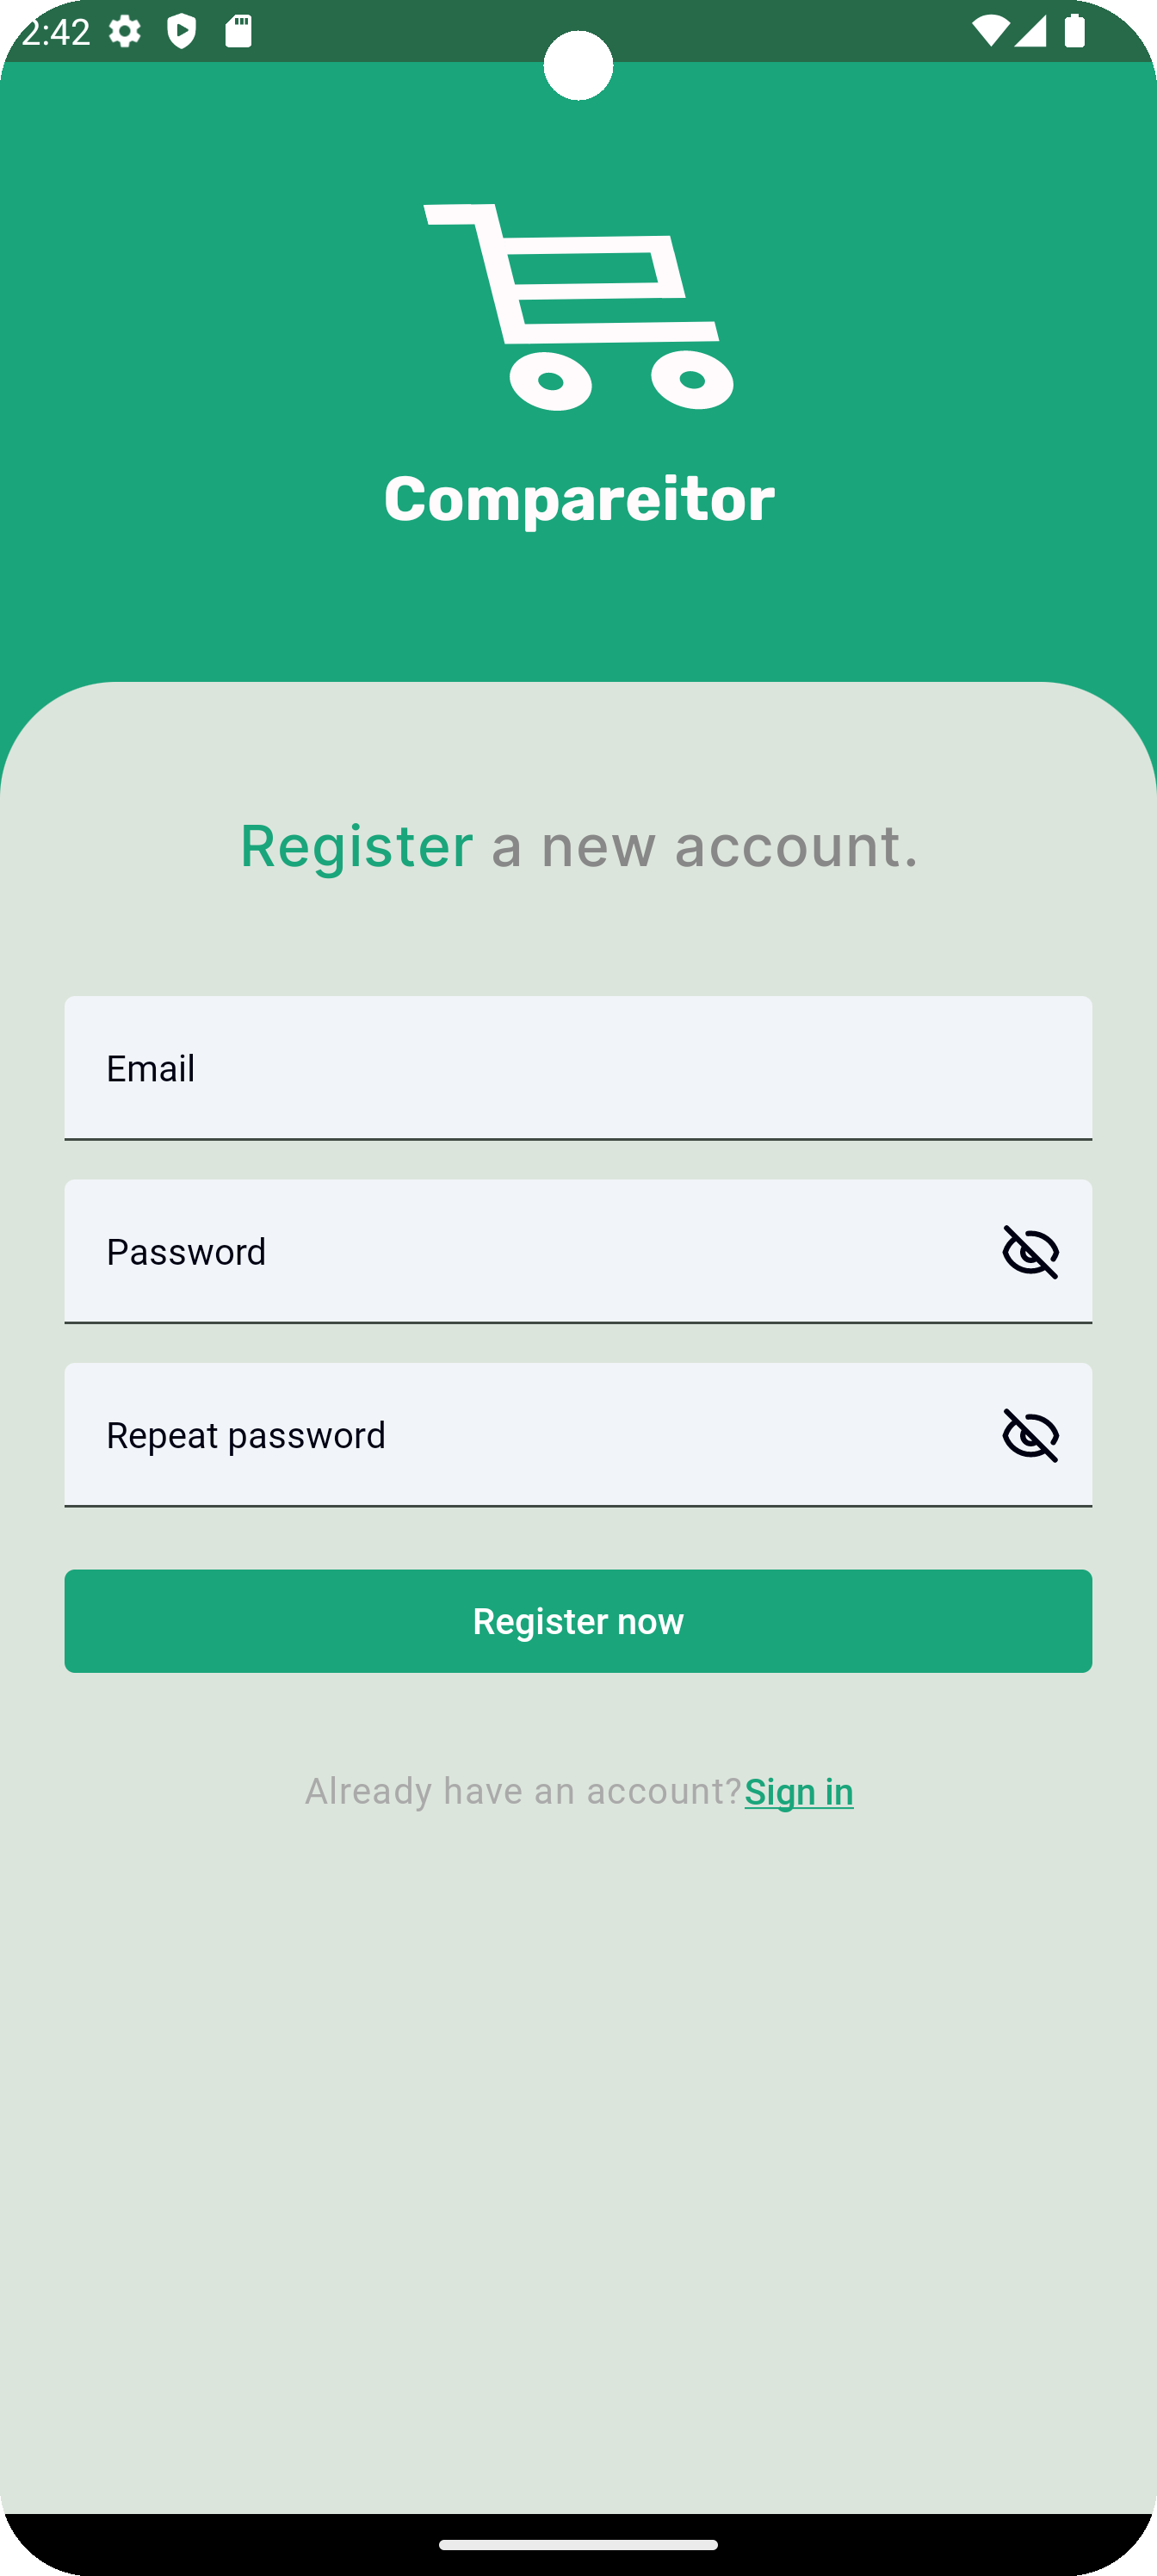
\includegraphics[width=0.55\textwidth,clip=true]{\register}
    \caption{Vista: Registro}
    \label{fig:Log-In}
\end{figure}

En la pantalla de inicio de sesión (véase \ref{fig:Log-In}), debajo del campo de contraseña, había un pequeño texto que decía \textbf{"Forgot Password"}. Al seleccionar esta opción, se nos lleva a una pantalla para recuperar la cuenta. Si hemos iniciado sesión con el método de correo/contraseña, se enviará un correo para recuperar la cuenta a la dirección que indiquemos.

\begin{figure}[H]
    \centering
	\includegraphics[width=0.55\textwidth,clip=true]{\recoverAccount}
    \caption{Vista: Recuperación de cuenta}
    \label{fig:Log-In}
\end{figure}

Al escribir el email nos llegará un correo como el siguiente:

\begin{figure}[H]
    \centering
	\includegraphics[width=1.00\textwidth,clip=true]{\recoverAccountCorreo}
    \caption{Vista: Recuperación de cuenta correo}
    \label{fig:Log-In}
\end{figure}

\begin{figure}[H]
    \centering
	\includegraphics[width=1.00\textwidth,clip=true]{\recoverAccountLink}
    \caption{Vista: Recuperación de cuenta link}
    \label{fig:Log-In}
\end{figure}

Al iniciar la aplicación, siempre se mostrará la pantalla de "Splash Screen". Esta pantalla actúa como un punto de espera mientras la aplicación se carga. En esta aplicación, la "Splash Screen" verifica que exista una conexión con la API para poder utilizar sus funcionalidades, tales como la búsqueda en diversas tiendas y la persistencia y recuperación de precios históricos de los productos buscados.

\begin{figure}[H]
    \centering
	\includegraphics[width=0.55\textwidth,clip=true]{\spashScreen}
    \caption{Vista: SpashScreen}
    \label{fig:Log-In}
\end{figure}

Cuando sé índice podremos si se ha podido conectar correctamente. 

Conexión exitosa

\begin{figure}[H]
    \centering
	\includegraphics[width=0.60\textwidth,clip=true]{\spalshScreenSuccess}
    \caption{Vista: SpashScreen exitosa}
    \label{fig:Log-In}
\end{figure}

Fallo en la conexión

\begin{figure}[H]
    \centering
	\includegraphics[width=0.63\textwidth,clip=true]{\spalshScreenError}
    \caption{Vista: SpashScreen fallo}
    \label{fig:Log-In}
\end{figure}

Al iniciar sesión dependiendo de cuál haya sido el método escogido, podremos ver en el apartado de usuario de tres maneras distintas:

\begin{figure}[H]
    \centering
	\includegraphics[width=0.60\textwidth,clip=true]{\annonSingin}
    \caption{Vista: Perfil-Autenticación anonima}
    \label{fig:Annon_Singin}
\end{figure}

\begin{figure}[H]
    \centering
	\includegraphics[width=0.68\textwidth,clip=true]{\correoSingin}
    \caption{Vista: Perfil-Autenticación con correo}
    \label{fig:Correo_Singin}
\end{figure}

\begin{figure}[H]
    \centering
	\includegraphics[width=0.68\textwidth,clip=true]{\googleSingin}
    \caption{Vista: Perfil-Autenticación con Google}
    \label{fig:Google_SingIn}
\end{figure}

La funcionalidad principal del programa, que es la búsqueda de productos, se encuentra en la sección de búsqueda. En esta sección, se puede ver un área para realizar las búsquedas, con las tiendas activadas por defecto, representadas con su logo en color. También incluye un selector (spinner) para elegir el modo de filtro de productos, que puede ser por precio o precio por cantidad. Al principio, la sección de resultados de búsqueda estará vacía.

\begin{figure}[H]
    \centering
	\includegraphics[width=0.55\textwidth,clip=true]{\productScreen}
    \caption{Vista: Busqueda}
    \label{fig:Google_SingIn}
\end{figure}

Al realizar una búsqueda, la barra de búsqueda mostrará un historial reciente de búsquedas y los productos correspondientes a la consulta actual. Si se desea aplicar diferentes filtros, los componentes de los filtros actuales se eliminarán y será necesario cambiar de vista y volver para reiniciar la búsqueda.

Los resultados de la búsqueda mostrarán los productos con su precio, precio por unidad, nombre, logo de la tienda a la que pertenecen, imagen del producto y sus ofertas, si las hubiera, además de un botón de favoritos.

\begin{figure}[H]
    \centering
	\includegraphics[width=0.52\textwidth,clip=true]{\productScreenResult}
    \caption{Vista: Búsqueda}
    \label{fig:Google_SingIn}
\end{figure}

En la vista de favoritos, se muestran los productos que hemos añadido a esta lista. Podemos eliminar un producto de favoritos seleccionando su icono de favoritos. Para actualizar la lista y ver los cambios, podemos cambiar de vista o refrescar la vista actual.

\begin{figure}[H]
    \centering
	\includegraphics[width=0.60\textwidth,clip=true]{\favoriteScreen}
    \caption{Vista: Favoritos}
    \label{fig:Google_SingIn}
\end{figure}

Al pulsar sobre un producto, ya sea en la búsqueda de productos o en la sección de favoritos, seremos redirigidos a una página dedicada al producto. En esta página, podremos acceder a una información más detallada, presentada de manera más amplia y legible.

Si estamos conectados a la API, tendremos la posibilidad de visualizar un gráfico que mostrará un historial de precios del producto. Además, podremos observar el precio medio a lo largo del tiempo, representado por una línea que atraviesa el gráfico. 

Los datos mostrados en el gráfico de la imagen son ilustrativos, ya que no se tiene ningún cambio de ningún producto actualmente y solo se vería el precio actual. 

\begin{figure}[H]
    \centering
	\includegraphics[width=0.47\textwidth,clip=true]{\productScreenSelected}
    \caption{Vista: Producto Seleccionado}
    \label{fig:ProductScreen}
\end{figure}

Podemos cerrar sesión pulsando el icono en la parte superior derecha. Al hacerlo, aparecerá una advertencia. Si confirmamos, seremos redirigidos a la vista de inicio de sesión.

\begin{figure}[H]
    \centering
	\includegraphics[width=0.60\textwidth,clip=true]{\cerrarSesion}
    \caption{Vista: Cerrar Sesión}
    \label{fig:Google_SingIn}
\end{figure}

% Nuevo capítulo
\chapter{Resultados y discusión}
\label{sec:resulObtenidos}

En este capítulo, examinaremos los resultados del desarrollo de la aplicación, destacando los problemas que se han resuelto. Discutiremos las limitaciones identificadas y evaluaremos si es posible resolverlas.

El proyecto enfrentó diversos desafíos durante su desarrollo, principalmente debido a la decisión de utilizar el framework Kotlin Multiplatform. Esta elección provocó retrasos significativos al inicio del proyecto. Además, la adopción de Compose para el desarrollo de la interfaz y la integración del nuevo sistema de librerías de android añadieron más complicaciones y contribuyeron a los retrasos en un tiempo ya ajustado.

Debido a la falta de tiempo, no fue posible desarrollar la funcionalidad de consultas con múltiples parámetros. En su lugar, se decidió enfocar los esfuerzos en las nuevas funcionalidades, asegurando que las características principales estuvieran completamente implementadas y optimizadas.

La aplicación no posee todas sus funcionalidades de manera autónoma y depende de la API para su funcionamiento completo. Esta dependencia limita su uso, pero ha permitido explorar nuevas tecnologías y metodologías. Además, ha abierto el camino hacia un formato de aplicación más escalable, orientado a un producto como servicio.

\blankpage

% Nuevo capítulo

\chapter{Conclusiones}

En este capítulo, se presentarán las conclusiones derivadas de las decisiones tomadas durante el proyecto, destacando los aspectos que han tenido éxito y aquellos que no. El objetivo es comprender las buenas prácticas aprendidas y evitar errores en proyectos futuros, buscando mejorar la eficiencia en el desarrollo.

\section{Informe post-mortem}

\subsection{Lo que ha ido bien}

\subsubsection{Implementación de Firebase}

 El uso de Firebase (véase la sección \ref{sec:Firebase}) ha significado una gran aportación para el proyecto, ya que ha facilitado la implementación principalmente de funcionalidades de inicio de sesión para los usuarios.

Gracias a Firebase, se ha implementado automáticamente el inicio de sesión con una cuenta de Google. Además, se ha facilitado el registro y autenticación de usuarios mediante correo electrónico y contraseña, permitiendo también la opción de restablecer la contraseña en caso de olvido. Asimismo, se ha añadido la posibilidad de que los usuarios inicien sesión en la aplicación de manera anónima.

Además, se ha añadido una funcionalidad de análisis que permite recopilar datos de la aplicación, como los productos más consultados, la ubicación desde donde se ha utilizado la aplicación y la cantidad de usuarios que se han conectado o registrado a lo largo del tiempo.


\subsubsection{Uso de buenas prácticas (clean code y arquitecturas de código)}

El uso de clean code y arquitecturas como la hexagonal en la API REST (véase la sección \ref{sec:Arquitectura Hexagonal}) ha sido fundamental. Estas buenas prácticas han agilizado el desarrollo de la aplicación, mejorando su mantenimiento a lo largo del tiempo, aumentando su legibilidad y facilitando su comprensión. Además, han permitido ahorrar tiempo en la refactorización de código y la corrección de errores. La implementación de logs claros a lo largo del programa también ha sido crucial para el desarrollo, proporcionando una mejor visibilidad y facilitando la identificación de problemas.

Se ha adoptado un enfoque orientado a la escalabilidad del proyecto, enfocando el desarrollo en clean architecture para permitir la adición de nuevas funcionalidades con mínimas modificaciones de código. Un ejemplo destacado es la API REST, que sigue una arquitectura hexagonal. Esta arquitectura permite añadir funcionalidades de manera sencilla al incorporar la lógica en los módulos de infraestructura y conectarlos a través de las interfaces de los puertos y los casos de uso. Este enfoque garantiza que cada componente sea independiente, con bajo acoplamiento y alta cohesión.

\subsection{Lo que ha ido mal}

	\subsubsection{Elección de un framework demasiado reciente}
 \label{sec:Mal-Kotlin-Multiplataforma}

\begin{itemize}

\item Para el desarrollo de la aplicación, se eligió la opción de usar Kotlin Multiplataforma. La principal motivación fue poder desarrollar aplicaciones multiplataforma, escribiendo el código una vez y ejecutándolo en Android, iOS, Escritorio e incluso Web con una única implementación.

%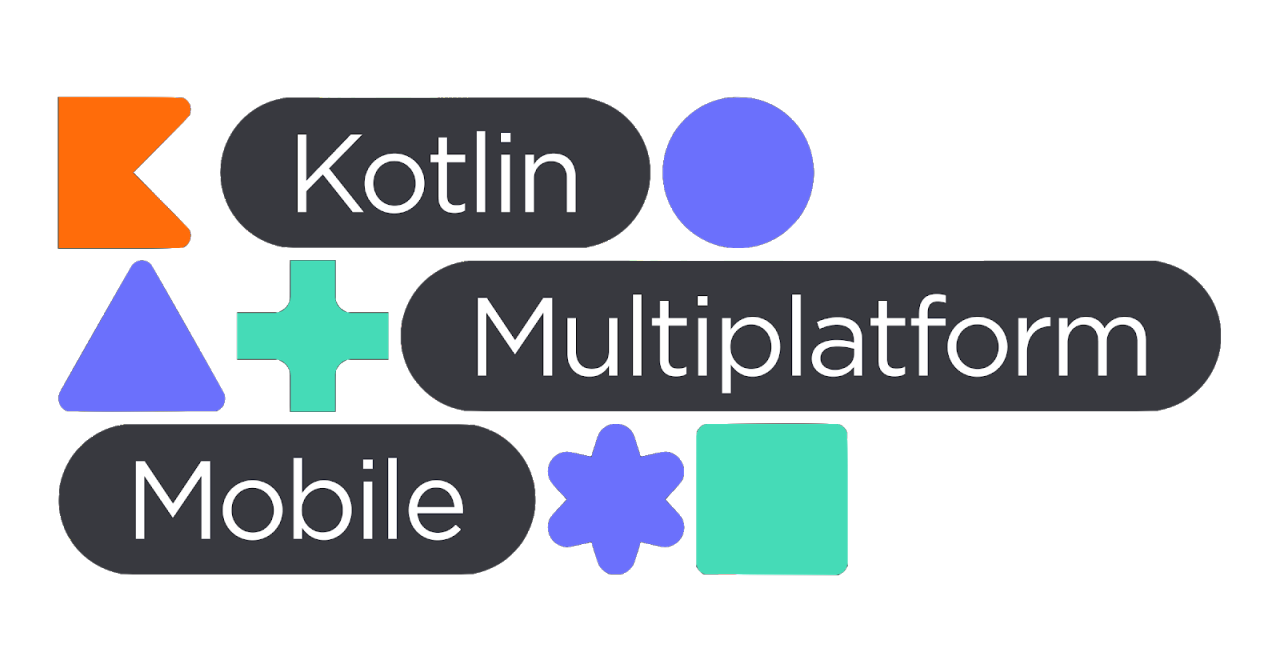
\includegraphics[width=\textwidth]{images/kotlin_multiplataform_logo.png}

\item La experiencia resultó ser muy tediosa, ya que encontrar información sobre las librerías y cómo usarlas es complicado. Existe un repositorio que posee una recopilación de librerías compatibles con Kotlin Multiplataforma en el repositorio \textit{Awesome Kotlin Multiplatform} \cite{kmp-awesome}, ya que las librerías de Kotlin regulares no son compatibles.

\item La importación también es diferente. Por ejemplo, la siguiente línea muestra cómo importar una librería en Gradle (Kotlin) y en Version Catalog (Kotlin-Multiplatform):

		            \begin{lstlisting}[caption={Ejemplo de importación de librerías en Gradle.}, label={alg:gradle.kts-examples}, language=Kotlin]
val voyagerVersion = "1.0.0"

implementation
("cafe.adriel.voyager:voyager-navigator:$voyagerVersion")
\end{lstlisting}

		            \begin{lstlisting}[caption={Ejemplo de importación de librerías en Version Catalog.}, label={alg:libs.versions.kts-examples}, language=Kotlin]
// libs.versions.toml					

voyager = "1.0.0"

voyager = { group = "cafe.adriel.voyager"  
name = "voyager-navigator", version.ref = "coil"}

//build.gradle.kts (Module :app)

implementation(libs.voyager)
\end{lstlisting}

\item La escasa documentación sobre cómo usar el framework, sumada a que la implementación de la interfaz gráfica era ligeramente distinta y tenía limitaciones en comparación con Android, llevó a abandonar la idea de desarrollar la aplicación en Kotlin Multiplataforma.

\end{itemize}

\subsubsection{Consultas poco estandarizadas e inconvenientes}

\label{sec:Mal-Consultas}

\begin{itemize}

\item Para el proyecto \titulotrabajo, se han llevado a cabo múltiples consultas mediante web scraping (véase la sección \ref{sec:WebScraping}). Sin embargo, cada página presenta sus propias particularidades, lo que demanda métodos distintos para extraer la información deseada.

Idealmente, habría sido beneficioso que todas las páginas dispusieran de una api que proporcionara un archivo json con los datos de los productos. Esto habría simplificado considerablemente la obtención de la información y mejorado el rendimiento de la aplicación. A pesar de ello, incluso en esos casos se ha tenido que filtrar el archivo json debido a su extensión, ya que su transformación completa a una clase de Kotlin no aportaría información relevante.

En aquellos casos en los que la api no proporciona un archivo json, se nos suministra el html puro de la página, el cual debemos filtrar según sus clases de css.

\item El principal inconveniente ha sido con la página web de Mercadona. En esta página, las consultas no funcionaban debido a que se necesita JavaScript para poder ver el contenido de la página. A continuación, dejo un ejemplo de lo que nos devuelve una consulta haciendo una petición GET:


    \begin{figure}[H]
				\centering
				\includegraphics[width=\linewidth]{\mercadonaPostman}
				\caption{Petición a la API de Mercadona}
				\label{fig:mercadonaPostman}
			\end{figure}

			\begin{figure}[H]
				\centering
				\includegraphics[width=\linewidth]{\mercadonaRequest}
				\caption{Respuesta de la petición a la API de Mercadona}
				\label{fig:mercadonaRequest}
			\end{figure}

\item Para llevar a cabo las consultas necesarias, se ha tenido que recurrir a Selenium (véase la sección \ref{sec:Selenium}). Esto ha representado un gran inconveniente, ya que no se puede ejecutar la biblioteca de manera nativa en Android. La solución que se ha encontrado es asociar las búsquedas a una API REST en un servidor (véase la sección \ref{sec:Springboot}).

\end{itemize}

\section{Trabajos futuros}

Han quedado pendientes los objetivos de realizar consultas con múltiples parámetros y desarrollar la aplicación de manera multiplataforma. En un futuro, se podría agregar la funcionalidad de búsqueda con múltiples parámetros. Aunque adaptar la aplicación a un framework multiplataforma es posible, esto dependerá del desarrollo y las librerías disponibles.

En un futuro, sería interesante que, además de buscar la información básica de los productos, también se pudiera recopilar la información nutricional de los mismos. Las tiendas de Día, Hipercor, Alcampo y Eroski poseen información nutricional de sus productos. Se podría recopilar esta información al igual que se ha hecho con los productos de otras tiendas. En los casos en que las tiendas no posean la información, los usuarios podrían proporcionarla.

Sería interesante autenticar a los usuarios mediante un método que verifique su identidad, como el que provee Firebase. Esto permitiría que los usuarios tengan una copia de sus ajustes, historial y productos favoritos, y puedan sincronizar la información entre dispositivos mediante la base de datos de la API.


\blankpage

\section{Diagrama de Flujo}

\begin{figure}[H]
    \centering
    \includegraphics[width=1.0\linewidth]{\diagramaFlujo}
    \caption{Diagrama de flujo de la aplicación}
    \label{fig:diagramaFlujo}
\end{figure}

\blankpage

%%%%%%%%%%%%%%%%%%%%%%%%%%%%%%% Bibliografía %%%%%%%%%%%%%%%%%%%%%%%%%%%%%%%
\phantomsection
\addcontentsline{toc}{chapter}{Bibliografía}

\begin{thebibliography}{99} % Ajusta el número según el máximo número de referencias
	\bibitem{kmp-awesome} Terrakok. \textit{Awesome Kotlin Multiplatform}, 2021. \href{https://github.com/terrakok/kmp-awesome}{Fuente}
	\bibitem{WebScraping} Geeksforgeeks. \textit{What is Web Scraping and How to Use It?}, 07 Mar, 2024 \href{https://www.geeksforgeeks.org/what-is-web-scraping-and-how-to-use-it/}{Fuente}
	\bibitem{Selenium WebDriver} El blog python \textit{Guía de Selenium WebDriver en Python para automatizar pruebas web} \href{https://elblogpython.com/tecnologia/guia-de-selenium-webdriver-en-python-para-automatizar-pruebas-web/}{Fuente}
	\bibitem{Super más barato} Súper más barato. \textit{Súper más barato} \href{https://supermasbarato.es/}{Fuente}
	\bibitem{Soysuper} Soysuper \textit{Soysuper más barato} \href{https://soysuper.com/}{Fuente}
    \bibitem{Firebase} Google \textit{Firebase} \href{https://firebase.google.com/}{Fuente}
    \bibitem{springboot-ibm} IBM \textit{¿Qué es Java Spring Boot?} \href{https://www.ibm.com/es-es/topics/java-spring-boot}{Fuente}
    \bibitem{springboot-baeldung} Baeldung \textit{REST with Spring Tutorial} \href{https://www.baeldung.com/rest-with-spring-series}{Fuente}
    \bibitem{jectack-compose} Android \textit{Compila mejores apps más rápido con Jetpack Compose} \href{https://developer.android.com/develop/ui/compose}{Fuente}
    \bibitem{arquitectura-hexagonal} Baeldung \textit{Organizing Layers Using Hexagonal Architecture, DDD, and Spring} \href{https://www.baeldung.com/hexagonal-architecture-ddd-spring}{Fuente}
    \bibitem{kotlin-multiplataform} Kotlin \textit{Kotlin Multiplatform} \href{https://kotlinlang.org/docs/multiplatform.html}{Fuente}
    \bibitem{retrofit} Baeldun \textit{Introduction to Retrofit} \href{https://www.baeldung.com/retrofit}{Fuente}
    \bibitem{mongodb} Builtin \textit{What Is MongoDB?} \href{https://builtin.com/data-science/mongodb}{Fuente}
    
    
\end{thebibliography}

% No expandir elementos para llenar toda la página
\raggedbottom
\afterpage{\blankpage}

% Fin del documento
\end{document}